% !TeX spellcheck = ru_RU

\chapter{Конструкторская часть}
В этом разделе будут разработаны схемы исследуемых алгоритмов, оценены трудоемкости в лучших и худших случаях.

\section{Разработка алгоритмов}
В этой части приведены схемы алгоритмов сортировки: пузырьком (\ref{fig:bubble_d}), пирамидальная (\ref{fig:heap_d}), блочная (\ref{fig:bucket_d}).
%\subsection{Сортировка пузырьком}
\begin{figure}[h]
	\centering
	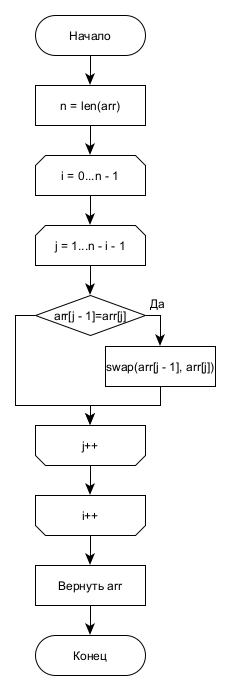
\includegraphics[scale = 0.5]{img/bubble_diag.png}
	\caption{Схема сортировки пузырьком}
	\label{fig:bubble_d}
\end{figure}
%\subsection{Пирамидальная сортировка}
\begin{figure}[h]
	\centering
	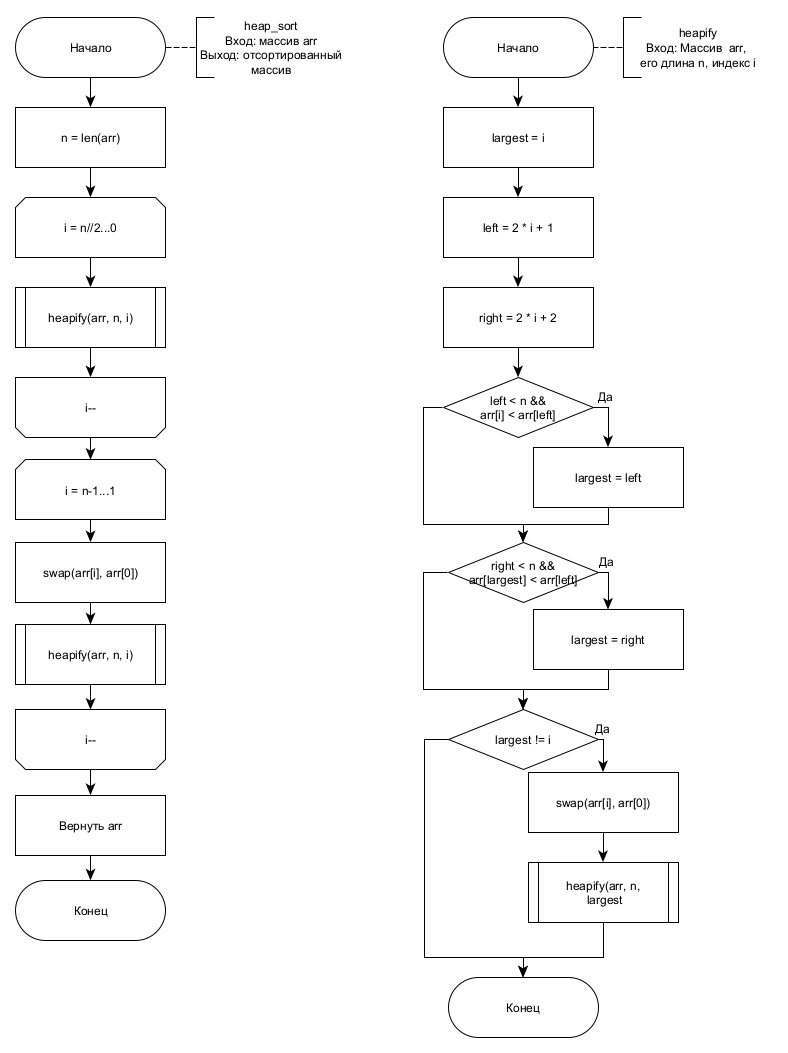
\includegraphics[scale = 0.5]{img/heap_diag.png}
	\caption{Схема пирамидальной сортировки (слева) и cхема подпрограммы heapify (справа)}
	\label{fig:heap_d}
\end{figure}
\clearpage
%\subsection{Блочная сортировка}
\begin{figure}[h]
	\centering
	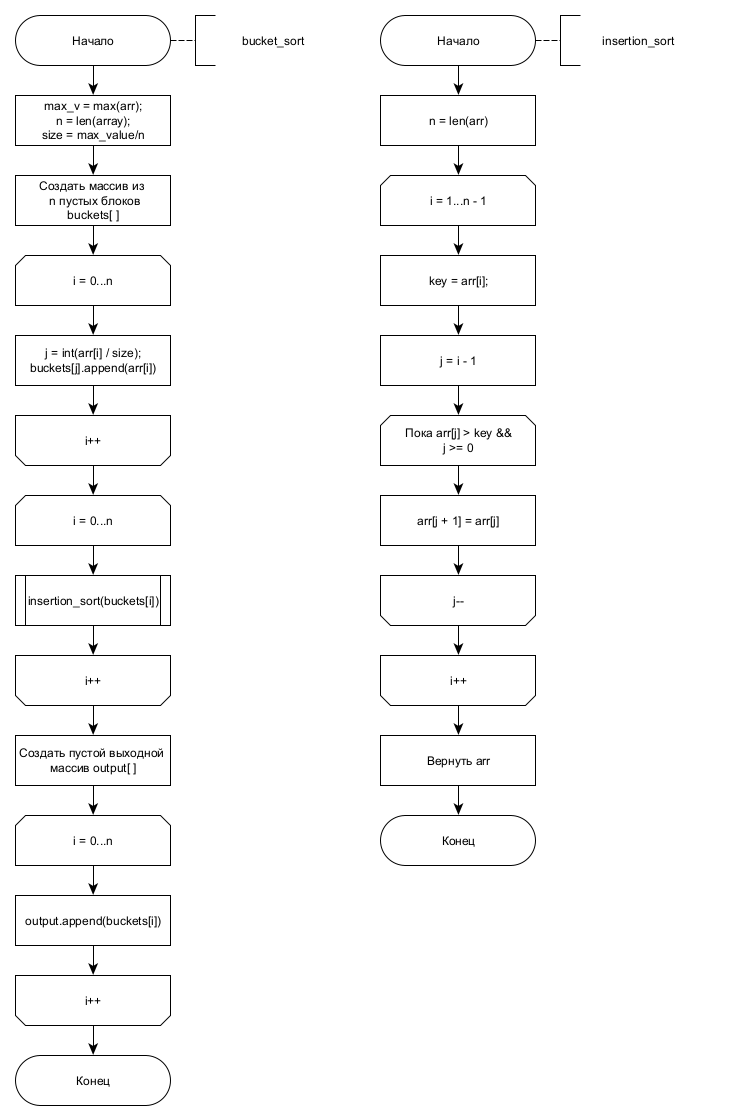
\includegraphics[scale = 0.45]{img/bucket_diag.png}
	\caption{Схема блочной сортировки (слева) и схема сортировки вставками, используемая как подпрограмма в алгоритме блочной сортировки (справа)}
	\label{fig:bucket_d}
\end{figure}
\clearpage
\section{Модель вычислений}

Для последующего вычисления трудоемкости введем модель вычислений \cite{model}:

\begin{enumerate}
	\item Операции из списка (\ref{for:opers}) имеют трудоемкость 1.
	\begin{equation}
		\label{for:opers}
		+, -, /, \%, ==, !=, <, >, <=, >=, [], ++, {-}-
	\end{equation}
	\item Трудоемкость оператора выбора \textit{if условие then A else B} рассчитывается, как (\ref{for:if}).
	\begin{equation}
		\label{for:if}
		f_{if} = f_{\text{условия}} +
		\begin{cases}
			f_A, & \text{если условие выполняется,}\\
			f_B, & \text{иначе.}
		\end{cases}
	\end{equation}
	\item Трудоемкость цикла рассчитывается, как (\ref{for:for}).
	\begin{equation}
		\label{for:for}
		f_{for} = f_{\text{инициализации}} + f_{\text{сравнения}} + N(f_{\text{тела}} + f_{\text{инкремента}} + f_{\text{сравнения}})
	\end{equation}
	\item Трудоемкость вызова функции равна 0.
\end{enumerate}

\section{Трудоемкость алгоритмов}

Пусть размер массивов во всех вычислениях обозначается как $N$.

\subsection{Алгоритм сортировки пузырьком}
Трудоемкость алгоритма сортировки пузырьком состоит из следующих элементов:
\begin{itemize}
	\item трудоемкость сравнения и инкремента внешнего цикла $i \in [1..N)$ (\ref{bubble:outer}).
	\begin{equation}
		\label{bubble:outer}
		f_{i} = 2 + 2(N - 1)
	\end{equation}
	\item суммарная трудоемкость всех срабатываний внутреннего цикла, количество итераций которого равномерно меняется в промежутке $[1..N-1]$, находится как сумма арифметической прогрессии (\ref{for:bubble_inner}).
	\begin{equation}
		\label{for:bubble_inner}
		f_{j} = 3(N - 1) + \frac{N\cdot(N - 1)}{2} \cdot (3 + f_{if})
	\end{equation}
	\item трудоемкость условия во внутреннем цикле (\ref{bubble:if}).
	\begin{equation}
		\label{bubble:if}
		f_{if} = 4 + \begin{cases}
			0, & \text{в лучшем случае}\\
			9, & \text{в худшем случае}\\
		\end{cases}
	\end{equation}
\end{itemize}

Трудоемкость в \textbf{лучшем} случае (\ref{bubble:best}).
\begin{equation}
	\label{bubble:best}
	f_{best} = \frac{7}{2} N^2 + \frac{3}{2} N - 3 \approx \frac{7}{2} N^2 = O(N^2)
\end{equation}

Трудоемкость в \textbf{худшем} случае (\ref{bubble:worst}).
\begin{equation}
	\label{bubble:worst}
	f_{worst} =  8N^2 - 8N - 3 \approx 8N^2 = O(N^2)
\end{equation}

%\subsection{Процедура heapify}
\subsection{Алгоритм пирамидальной сортировки}
Перед тем как дать оценку трудоемкости алгоритма пирамидальной сортировки, дадим оценку трудоемкости процедуры heapify, используемой в указанном алгоритме сортировки.

Заметим, что высота n-элементной пирамиды равна $\lfloor \lg{n}\rfloor$. Тогда процедура heapify для пирамиды размером n рекурсивно вызывает себя не более чем $\lfloor \lg{n}\rfloor$ раз.
С учетом этого факта можно дать оценку трудоемкости рассматриваемой процедуры.

Трудоемкость подпрограммы heapify в \textbf{лучшем} случае (\ref{h:best}).
\begin{equation}
	\label{h:best}
	f_{best} = 16 = O(1)
\end{equation}

Трудоемкость подпрограммы heapify в \textbf{худшем} случае (\ref{h:worst}).
\begin{equation}
	\label{h:worst}
	f_{worst} = 16 + 9 + 25\lfloor \lg{n}\rfloor \approx 25\lfloor \lg{n}\rfloor = O(\lfloor \lg{n}\rfloor)
\end{equation}
\newpage
%\subsection{Алгоритм пирамидальной сортировки}
Трудоемкость алгоритма пирамидальной сортировки состоит из следующих элементов:
\begin{itemize}
	\item трудоемкость сравнения и инкремента первого цикла $i \in [N/2...0]$ (\ref{heap:first}).
	\begin{equation}
		\label{heap:first}
		f_{i} = 3 + 2(N/2)
	\end{equation}
	\item трудоемкость второго цикла (без учета вызовов подпрограммы heapify)\newline$j \in [N-1...0)$ (\ref{heap:second}).
	\begin{equation}
		\label{heap:second}
		f_{j} = 3 + 2(N-1)
	\end{equation}
	\item суммарная трудоемкость вызовов heapify в двух циклах $i \in [N/2...0]$ и $j \in [N-1...0)$  (\ref{heap:h}).
	\begin{equation}
		\label{heap:h}
		f_{summ_{heapify}} = 16 + (N/2 + N - 1)f_{heapify}, 
	\end{equation}
	где трудоемкость $f_{heapify}$ равна (\ref{heap:h1}).
	\begin{equation}
		\label{heap:h1}
		f_{heapify} = \begin{cases}
			16, & \text{в лучшем случае}\\
			25 + 25\lfloor \lg{n}\rfloor, & \text{в худшем случае}\\
		\end{cases}
	\end{equation}
\end{itemize}


Трудоемкость в \textbf{лучшем} случае (\ref{heap:best}).
\begin{equation}
	\label{heap:best}
	f_{best} = 22 + 16(N/2 + N - 1) + 2(N-1+N/2) \approx 27N = O(N)
\end{equation}

Трудоемкость в \textbf{худшем} случае (\ref{heap:worst}).
\begin{equation}
	\begin{split}
		\label{heap:worst}
		f_{worst} &=  22 + (N/2 + N - 1)(25 + 25\lfloor \lg{n}\rfloor) + 2(N-1+N/2)
		\approx \\&\approx \frac{75}{2}N\lfloor \lg{n}\rfloor = O(N\lg{n})
	\end{split}
\end{equation}

\subsection{Алгоритм блочной сортировки}
%\subsection{Алгоритм сортировки вставками}

Перед тем как дать оценку трудоемкости алгоритма блочной сортировки, дадим оценку трудоемкости сортировки вставками, используемой в алгоритме блочной сортировки в качестве подпрограммы.

Трудоемкость алгоритма сортировки вставками состоит из следующих элементов.
\begin{itemize}
	\item трудоемкость внешнего цикла $i \in [1..N)$ (без учета внутреннего цикла)(\ref{for:isort_outer}):
	\begin{equation}
		\label{for:isort_outer}
		f_{i} = 2 + 2(N - 1) + 7(N-1)
	\end{equation}
	\item суммарная трудоемкость всех срабатываний внутреннего цикла, количество итераций которого меняется в промежутке $[1..N-1]$ (\ref{for:isort_inner}):
	\begin{equation}
		\label{for:isort_inner}
		f_{while} = \begin{cases}
			(N-1)\cdot4, & \text{в лучшем случае}\\
			(N-1)\cdot10(N - 1), & \text{в худшем случае}\\
		\end{cases}
	\end{equation}
	
\end{itemize}

Трудоемкость в \textbf{лучшем} случае (\ref{for:isort_best}).
\begin{equation}
	\label{for:isort_best}
	f_{best} = 9N - 3 + 4N - 4\approx 13N = O(N)
\end{equation}

Трудоемкость в \textbf{худшем} случае (\ref{for:isort_worst}).
\begin{equation}
	\label{for:isort_worst}
	f_{worst} = 10N^2 - 20N - 10 + 9N - 3\approx 10N^2 = O(N^{2})
\end{equation}

%\subsection{Алгоритм блочной сортировки}

Трудоемкость алгоритма сортировки вставками состоит из следующих элементов:
\begin{itemize}
	\item трудоемкость первого цикла (создание N пустых блоков)$i \in [0...N)$ (\ref{bucket:first}).
	\begin{equation}
		\label{bucket:first}
		f_{1} = 2 + 2N + N
	\end{equation}

	\item трудоемкость второго цикла (занесение чисел в блоки)$i \in [0...N)$ (\ref{bucket:second}).
	\begin{equation}
		\label{bucket:second}
		f_{2} = 2 + 2N + 5N
	\end{equation}

	\item трудоемкость третьего цикла (применение сортировки вставками к каждому блоку)$i \in [0...N)$. При этом следует учитывать, что трудоемкость сортировки i-го блока зависит не от общей длины массива N, а от числа $n_{i} \leq N$ элементов, попавших в i-ый блок(\ref{bucket:second}):
	\begin{equation}
		\label{bucket:insert}
		f_{3} = 2 + 2N + \sum{k=0}^{N-1}f_{ins_{k}}
	\end{equation}, где $f_{ins_{k}}$ --- переменная трудоемкость сортировки k-го блока, зависящая от длины $n_k$.
\end{itemize}

При определении трудоемкости блочной сортировки в лучшем и худшем случае следует учитывать, что по аналогии с хэш-таблицами, наилучший результат будет достигаться при наименьшем количестве "коллизий" --- попаданий нескольких чисел в один и тот же блок. Очевидно, что при длине массива N и количестве блоков, равном N, наилучший случай достигается, когда в каждый блок попадает ровно 1 число и трудоемкость сортировки вставками каждого блока является тривиальной (O(1)). Напротив, наихудший результат достигается при попадании всех N элементов массива в один блок. Тогда суммарная сложность сортировки всех блоков равна сложности сортировки входного массива алгоритмом сортировки вставками.

Трудоемкость в \textbf{лучшем} случае (\ref{for:heap_best}).
\begin{equation}
	\label{for:heap_best}
	f_{best} = 13N + 6 + (13N - 7) \approx 26N = O(N)
\end{equation}

Трудоемкость в \textbf{худшем} случае (\ref{for:heap_worst}).
\begin{equation}
	\label{for:heap_worst}
	f_{worst} = 13N + 6  + (10N^2 - 11N - 10 - 3) \approx 10N^2 = O(n^2)
\end{equation}

\section*{Вывод}
На основе теоретических данных, полученных в аналитическом разделе были построены схемы исследуемых алгоритмов, посчитаны теоретические трудоемкости алгоритмов в лучших и худших случаях.